\chapter{Experiments and results}\label{chap:exp_res}
This chapter evaluates the proposed method on a toy example which consists of $128$ by $128$ pixel images with $6$ to $10$ disks with radii between $6$ and $8$ that are non overlapping but might be touching. The images are single channel and the disks are seperating themselves from the background by phase shiftet interfering frequencies. An example is depicted in figure \ref{fig:exmpl}.

\begin{figure}[ht!]
	\centering
	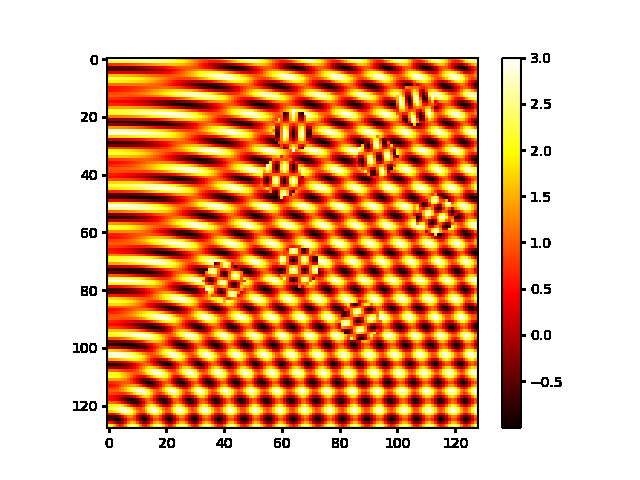
\includegraphics[width=.5\textwidth]{figures/plots/raw.png}
	\caption{Example raw image}
	\label{fig:exmpl}
\end{figure}

The incentive is to do instance segmentation for the disks. That is labeling each of the discs in a unique object ID. There where some foreground background segmentations created along with the raw data. This segmentations are used to train the embedding network as described in section \ref{seg:pip_embed}. Note that training the embedding network on foreground background images with contrasive loss generates two clusters only in the embedding space, one for foreground and one for background. For the node features it is only important to be distinctive between those two classes because that is all it needs for a merge/unmerge decision.\\
The pixel embeddings are visualized by their values in the first three principal components (see section \ref{sec:pca}) of the whole set of pixel embeddings. The three values per pixel are converted to an rgb image. Note that for most trained pixel embeddings the majority of the information is contained within their first three principal components. In figure \ref{fig:pixembeddings} this method of visualization was used on the pixel embeddings of the example image.\\

\begin{figure}[ht!]
	\centering
	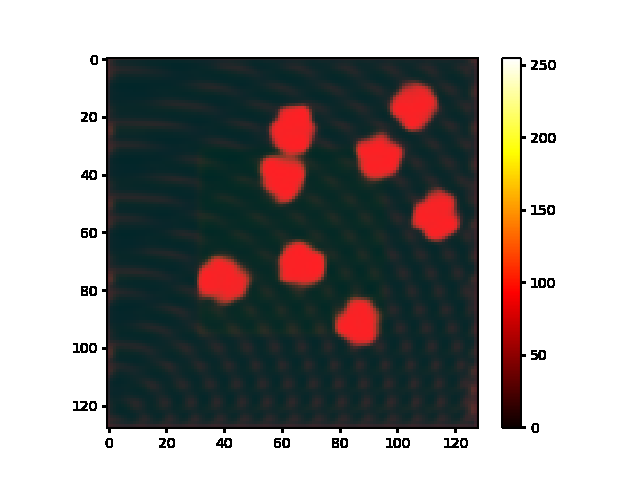
\includegraphics[width=.5\textwidth]{figures/plots/pix_embeddings.png}
	\caption{Values in first three principal components of pixel embeddings}
	\label{fig:pixembeddings}
\end{figure}

The affinities that are needed for the mutex watershed algorithm are calculated based on the fist and second gradient of the raw data for short range attractive edges. For long lange repulsive edges the concept of the first and second gradient computation by forward differences is used for pixelwise differences between the incidental pixels of the long range edges.\\
The algorithm mainly tested on this data operates in a continuous action space where the actor predicts mean and variance for a normal distribution sitting on every edge of the superpixel graph. The rewards are calculated in a supervised fashion based on the ground truth segmentation and in a unsupervised fashion based on the number of objects the knowledge that they are discs and their approximate radius.
\subsection{Supervised training}
For the supervised method a reward per subgraph is obtained by the dice score over the set of edges in the subgraph and the groundtruth edges obtained by evaluating if the larger parts of the incidental superpixels are of different classes in the grount truth segmentation. The larger parts are taken here because it is not guaranteed that the superpixels do not cross edges in the ground truth segmentation.\\
The setup includes a replay buffer storing $100$ experience tuples of $(s_t, a_t, r_{t+1}, s_{t+1})$. Initially experience is sampeld until the buffer is full. Then after each collected experience tuple there are 10 optimization steps performed on sampled experience tuples. Optimization is done by stochastic gradient descent on mini batches of size $10$ using the Adam optimizer, introduced in \cite{kingma2014adam}. For the setting where the embedding network was "warmed up" on the image - ground truth pairs prior to training the embedding networks parameters remain fixed after and no more optimization is performed on them. The optimization of the embedding network by the actors optimizer and loss function has been tested ended in messy embeddings. This can be related to the high variance in the actors loss function.\\
An example of the result using the per subgraph dice score as a reward is shown in figure \ref{fig:resa_dicebel}.\\

\begin{figure}[ht!]
	\centering
	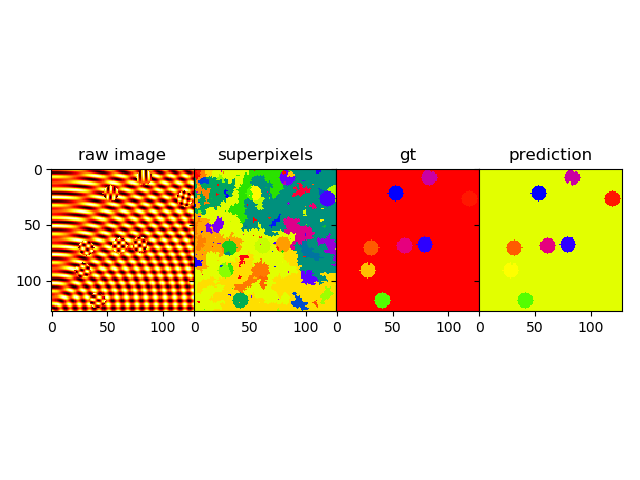
\includegraphics[width=.7\textwidth]{figures/plots/results_dice_reward.png}
	\caption{Result using the dice reward after $80000$ optimization steps on mini batches of size $10$. The gt image was obtained by computing the multicut based on the ground truth edges}
	\label{fig:resa_dice}
\end{figure}

The values in their first $3$ principal components of the edge features, extracted from one of the critics networks are displayed in figure \ref{fig:res_edge_embed}. After training they clearly carry the ground truth information in them.\\

\begin{figure}[ht!]
	\centering
	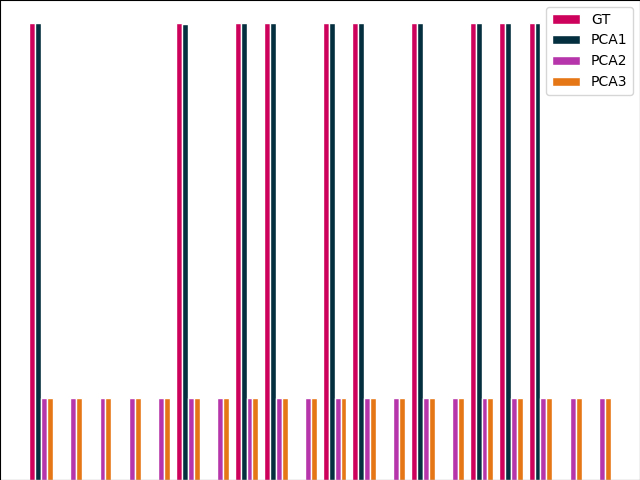
\includegraphics[width=.5\textwidth]{figures/plots/edge_embeddings.png}
	\caption{Visualization of the values of the edge features is their first $3$ principal components (PCA1-3) and the ground truth edge values (GT) after training with the dice rewards for $80000$ optimization steps on mini batches of size $10$.}
	\label{fig:res_edge_embed}
\end{figure}

The emperically predicted means of the actor network are visualized by histograms in figure \ref{fig:pred_means}. The prediction sepearates nicely and shows the class inbalance of $0$ and $1$ edges. The separation also shows, that the there is almost no uncertainty in the predictions anymore, leaving the multicut algorithm with a very simple task.

\begin{figure}[ht!]
	\centering
	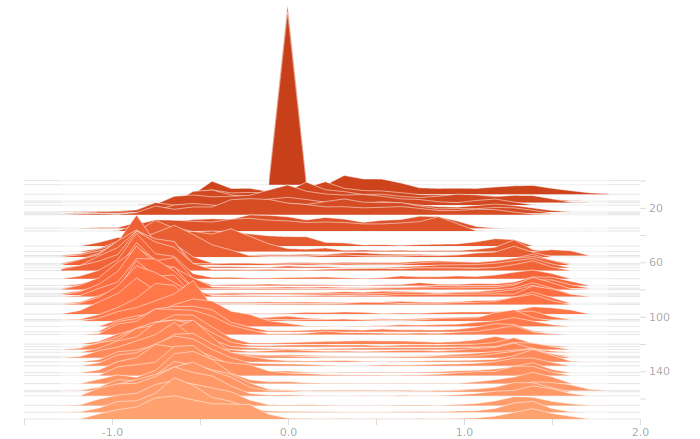
\includegraphics[width=.7\textwidth]{figures/plots/logit_means_hist.png}
	\caption{History of predicted means for the policy (supervised reward setting)}
	\label{fig:pred_means}
\end{figure}

\subsection{Unsupervised training}

Since there is still some ground truth involved in the warmup training for the feature extractor, this setup cannot be considered fully unsupervised. But there is no more ground truth involved in obtaining the rewards which results in a large loss of supervision. The rewards are calculated locally on superpixel basis as well as globally in the following fashion.\\
From the segmentation obtained from the multicut based on the sampled action values objects larger than $32^2$ pixels are considered background and all remaining objects are considered foreground. If there are too few foreground objects (number of objects is part of prior knowledge), all superpixels covered by background objects receive a negative reward. If there are too many objects, all the superpixel covered by foreground objects receive a negative reward.\\
A score for the shape of the foreground objects can be obtained using the Heugh transform for circles (see section \ref{ssec:heugh_tf}). The Heugh transform of the corresponding radii (part of prior knowledge) is applied on the edge image of the resppective segmentation. All superpixels that are covered by discs that are drawn at the peaks of the Heugh transform above a threshold of $0.8$ receive a positive reward dependend on the value in the Heugh transform at their respective peak.\\
In a final step the rewards are collected over each subgraph and averaged to a single value. This method indeed generates quite noisy rewards but the proposed pipeline was drafted to compensate for that.\\
Figure \ref{fig:resa_dice} shows an example of the results where the policy was trained under the unsupervised rewards.

\begin{figure}[ht!]
	\centering
	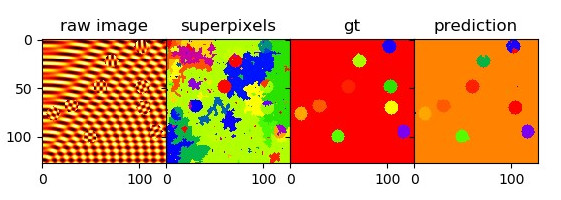
\includegraphics[width=.8\textwidth]{figures/plots/res_unsup.jpeg}
	\caption{Result using the unsupervised reward after $80000$ optimization steps on mini batches of size $10$. The gt image was obtained by computing the multicut based on the ground truth edges}
	\label{fig:resa_dice}
\end{figure}
As the histogram of the predicted means for the policy in figure \ref{fig:resa_dice} shows, the predictions are not so clearly separated into means that are larger than $1$ or smaller than $0$ as is the case in the supervised setting. This can be attributed to the noisy rewards and leaves the multicut algorithm with a harder problem than in the supervised setting.\\

\begin{figure}[ht!]
	\centering
	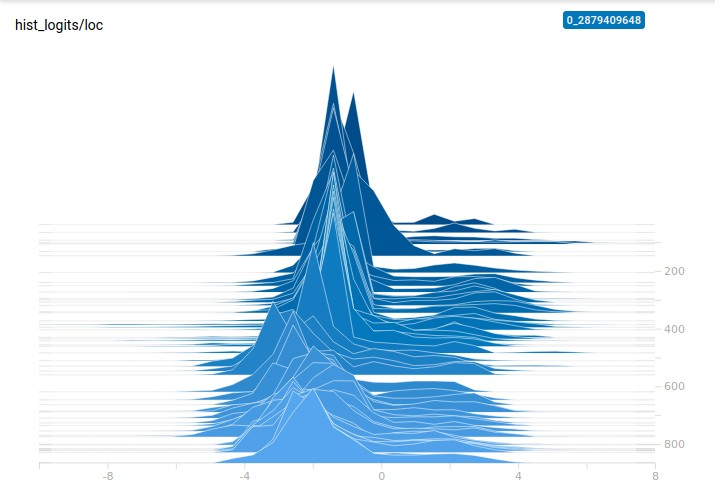
\includegraphics[width=.6\textwidth]{figures/plots/hist_unsup.jpeg}
	\caption{History of predicted means for the policy (unsupervised reward setting)}
	\label{fig:resa_dice}
\end{figure}

\subsubsection{Data conformity}
Supervised learning naturally provides a strict relation to the input data because the ground truth sample directly depends on the raw data.\\
Unsupervised learning typically needs a data term that encourages the solution to be close to the input data. The data term in this pipeline are the affinities and therefore the superpixel segmentation. The policy network learns ideally to distinguish between disc and non-disc superpixels. In an unfortunate case however it also could learn to build disks out of background superpixels. This would be the case if the shape of each superpixel is encoded in the pixel embeddings and the policy network learns to build discs based only on this shapes.


